% ---------------------------------------------------------
% Project: PhD KAPPA
% File: background.ipd.tex
% Author: Andrea Discacciati
%
% Purpose: Section IPD (background)
% ---------------------------------------------------------

\section{Survival analysis of primary data}
\label{section:saipd}

Survival analysis refers to the analysis of time from a specific time point until the occurrence of a well-defined event (survival time).\footnote{The terms `event', `outcome', and `disease' are equivalent and therefore they are used interchangeably in this thesis.} A unique characteristic of survival data is that observations may be censored --- that is, for some study individuals the event time is unknown. There are different censoring mechanisms, but right-censoring --- arguably the most common in epidemiologic studies --- is the only type of censoring considered in this thesis. Furthermore, we will make the assumption that survival time and censoring time are independent, possibly conditional on a vector of known, fixed covariates.

With no censoring, survival time can be analyzed as any other numeric variable, for example using Wilcoxon's rank-sum test or standard quantile regression. 
When censoring is present, a number of statistical tools is available to deal with this mechanism. However, one should always remember that the ultimate goal is to describe the distribution of survival time, and how this is affected by a vector of covariates. 

Lastly, the term `primary data' (or `individual patient data') refers to the availability of raw data for each participant in an epidemiologic study or clinical trial, as opposed to aggregated data.

\subsection{Basic statistical concepts}
\label{section:basicstatconcepts}

The statistical concepts introduced in this section are standard and therefore only a brief overview will be given. See for example \citet{kleinbaum_survival_2012} for a more rigorous and detailed exposition.

Let $T$ be a continuous, non-negative random variable with probability density function (p.d.f.) $f(t)$, and cumulative density function (c.d.f.) $F(t) = \Pr(T \le t)$, which gives the probability that the event has occurred by time $t$. Usually, one observes the possibly right-censored random variable $Y = \min(T, C)$, where $C$ is the censoring random variable. In addition to the p.d.f. and the c.d.f., there are three  alternative but equivalent  functions to describe the distribution of $T$. These are the survival function, the hazard function, and the cumulative hazard function.

The survival function $S(t)$ gives the probability that the survival time is larger than $t$ --- that is, the probability of being event-free at time $t$. It is a non-decreasing function of $t$ and can take values between 0 and 1. $S(t)$ is equal to 1 minus the c.d.f.:
\begin{equation}
S(t) = \Pr(T > t) = 1 - F(t) = \int_t^{+\infty}f(s)ds.
\label{eq:survivalfunction}
\end{equation}

A common non-parametric estimator for the survival function is the Kaplan-Meier product-limit estimator \citep{kaplan_nonparametric_1958}.

A different characterization of the distribution of $T$ is given by the hazard function $h(t)$, which is defined as:
\begin{equation}
h(t) = \lim_{dt \rightarrow 0} \frac{\Pr(t < T \le t + dt | T > t)}{dt}.
\label{eq:hazardrate}
\end{equation} 

The numerator of the hazard function is the conditional probability that the event of interest will happen in the time interval $(t,t+dt)$, given that it has not occurred before. The denominator is the width $dt$ of such a time interval. By dividing the first by the second, one obtains the event rate per unit of time, and taking the limit as $dt$ goes to 0, the instantaneous event rate. Therefore, $h(t)dt$, for an infinitesimal $dt$, is akin to the conditional probability that the event will occur in the time interval $(t,t+dt)$ given $S(t)$. However, the hazard itself is not a probability (and in fact it is not bounded between 0 and 1). The key feature of the hazard function is its conditional nature. Contrast, for example, the unconditional probability, for all the men born on a given year, of dying after 40 years of age [$S(40)$], with the probability of dying in the time interval $(39 < T \le 40 \textrm{ years } | \textrm{ alive at 39 years})$. For example, $S(40)$ was estimated to be around 60\% for men born in 1861 in Sweden. However, given survival up to 39 years of age, the probability of being alive at age 40 years was much higher, roughly 98\% \citep{scb_cohort_2010}.

Lastly, the cumulative hazard function is the integrated hazard function:
\begin{equation*}
H(t)=\int_0^t h(s)ds.
\end{equation*}

All the functions described above are mathematically related and in particular,
\begin{align}
S(t) &= \exp\left(-H(t)\right) = \exp\left(-\int_0^t h(s)ds\right). \label{eq:SfromH}
\end{align}

\subsection{The proportional-hazards approach to survival modeling}
\label{sec:phapproach}

In the previous section we focused on how to characterize the distribution of $T$. However, a major objective in epidemiologic research is to describe the variation in the distribution of $T$ --- and therefore in survival --- among individuals, given a vector of covariates. Different ``classical'' approaches to survival modeling are available, the most common probably being Accelerated Failure Time models and proportional-hazards (PH) models. An additional  approach was recently introduced by \citet{royston_flexible_2002}.\footnote{Royston-Parmar models include, but are not limited to, PH models.} In this section we will give a brief overview of the PH model. The literature on this topic is enormous and the reader can refer for example to \citet{therneau_modeling_2000}, \citet{kalbfleisch_statistical_2002}, and \citet{vanhouwelingen_cox_2013} for a more complete discussion.

\subsubsection{The proportional-hazards model}
The PH model focuses directly on the hazard function. In particular, the hazard at time $t$, for a given individual $i$ with covariate vector $\mathbf{x}_i=(x_{i1},\ldots,x_{ik})$ (not including a constant), is assumed to be:
\begin{equation}
h_i(t|\mathbf{x}_i) = h_0(t)\exp\left(\mathbf{x}_i^\top\boldsymbol{\beta}\right),
\label{eq:phmodels}
\end{equation}
where $ h_0(t)$ is the baseline hazard for all individuals with $\mathbf{x}_i = \left(0,\ldots,0\right)$, $\boldsymbol{\beta} = \left( \beta_1,\ldots,\beta_k \right)$ is the vector of unknown model coefficients, and $\exp\left(\mathbf{x}_i^\top\boldsymbol{\beta}\right)$ is a proportional (multiplicative) increase or reduction of the baseline hazard associated with the covariates $\mathbf{x}_i$ --- that is, the Hazard Rate Ratio (HRR). Of note, this proportional increase or reduction in baseline hazard is constant over $t$. In other words, PH models assume that the relative effect of a covariate is the same at all time points.

An immediate consequence of models written in the form of equation (\ref{eq:phmodels}), is that the cumulative hazards are proportional too. In fact, integrating both sides of the equation from 0 to $t$ gives the following result:
\begin{equation}
H_i\left(t|\mathbf{x}_i\right) = \int_0^t h_0(s)\exp\left(\mathbf{x}_i^\top\boldsymbol{\beta}\right)ds = H_0(t)\exp\left(\mathbf{x}_i^\top\boldsymbol{\beta}\right).
\label{eq:phcumhazard}
\end{equation}
Moreover, given equation (\ref{eq:SfromH}), the following relation for the survival function is immediately obtained:
\begin{equation}
S_i(t|\mathbf{x}_i) = S_0(t)^{\exp\left(\mathbf{x}_i^\top\boldsymbol{\beta}\right)}.
\label{eq:phmodelssurv}
\end{equation}

This important result says that, for PH models, the effect of the covariate vector $\mathbf{x}_i$ on the survival function is to raise $S_0(t)$ (the baseline survival function) to a power equal to the constant $\exp\left(\mathbf{x}_i^\top\boldsymbol{\beta}\right)$. As \citet[pg.~118]{kalbfleisch_statistical_2002} pointed out ``note that the assumed model constraints the estimates so that one survivor function dominates the other. Such graphs can give a misleading impression that one of the treatments is consistently preferable and suggest significant differences even when they are not present.''

%TODO: Left truncation?

\subsubsection{Time-dependent coefficients}
The PH model lends itself to extensions, such as time-varying covariates and time-dependent coefficients. In particular, time-dependent coefficients are useful to relax the assumption of proportionality of the hazards over time. To accommodate time-dependent coefficients, the PH model can be rewritten as:
\begin{equation}
h_i(t|\mathbf{x}_i) = h_0(t)\exp \left(\mathbf{x}_i^\top\boldsymbol{\beta}(t)\right),
\label{eq:timedepph}
\end{equation}
and the time-dependent coefficients are modeled using $b$ transformations of time. For example, suppose that only one coefficient $\beta(t)$ is included in the model, then 
\begin{equation}
\beta(t) = \sum_{j=1}^b \gamma_j g_j(t).
\label{eq:timevcoef}
\end{equation}

This extended model --- sometimes referred to as `extended PH model' or `general hazard rate model' ---  implies that the HRR is free to vary over time (time-dependent HRR). Another consequence is that the simple equation (\ref{eq:phmodelssurv}) does not longer apply, as the coefficients are now a function of time and therefore they cannot be taken out of the integral in equation (\ref{eq:phcumhazard}). The survival curve for the $i$-th individual is now given by:
\begin{equation}
S_i(t|\mathbf{x}_i) = \exp\left(-\int_0^t h_0(s)\exp \left(\mathbf{x}_i^\top\boldsymbol{\beta}(s)\right) ds \right).
\label{eq:tvphmodelssurv}
\end{equation}

Calculation of the survival curve is still possible, but is now more complicated. The integral in equation (\ref{eq:tvphmodelssurv}) can be derived analytically (in simple parametric situations) or numerically, as a cumulative sum of predictions. The latter approach is described in detail by \citet[section 4]{carstensen_demography_2005}. The complexity in the calculation of model-based survival curves is certainly a drawback of PH models with time-dependent coefficients. At the same time, one should keep in mind that these models put the focus on the HRR, which on the other hand is quite simple to calculate even in the presence of time-dependent coefficients \citep{heinzl_gaining_1997}.

The consequences on the HRR of the omission of time-dependent coefficients  when actually needed are numerous in the literature \citep[see, for example,][]{royston_use_2011, uno_moving_2014}. Figure \ref{fig:phnophsurvcurve}, on the other hand, shows an example of such consequences on model-based predicted survival curves. In particular, in panel A the hazards were forced to be proportional [equation (\ref{eq:phmodelssurv}) for the survival curves applies], whereas in panel B this assumption was relaxed by including a time-dependent coefficient [equation (\ref{eq:tvphmodelssurv}) for the survival curves applies].

\begin{figure}[p]
\begin{center}
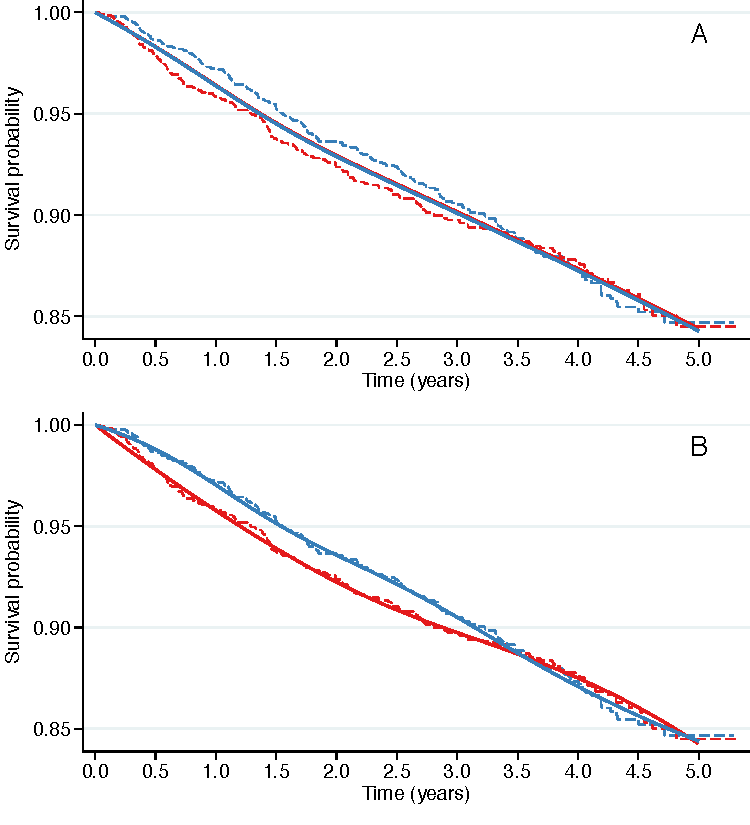
\includegraphics[width=\linewidth]{figures/phnophsurvcurve.pdf}
\end{center}
\caption[Survival curves from proportional-hazards models]{Consequences of the violation of the PH assumption on the predicted survival curves. In panel A, a PH model without time-dependent coefficients was employed. The model-based predicted survival curves for women in the active treatment (red solid line) and in the placebo arm (blue solid line) were far off from the corresponding non-parametric Kaplan-Meier estimates (dashed lines). In panel B, the time-dependent coefficient for the binary variable indicating the treatment group was modeled using restricted cubic splines with 5 knots. As a result, the model-based predicted survival curves  followed closely the corresponding non-parametric estimates. Note how in panel B the model-based survival curves cross after around 3.5 years, following the behavior of the Kaplan-Meier estimates. See \citet{hulley_randomized_1998} for more information about the data.}
\label{fig:phnophsurvcurve}
\end{figure}

\subsubsection{Model fitting}
There are different possible approaches to fitting hazard rate models. %, and the ubiquitous Cox model is just one of them. 

The first is the `pure' parametric approach, where the time variable $T$ is assumed to follow a specific distribution. Consequently, a specific functional form is assumed for the baseline hazard $h_0(t)$. Examples of distributions used to characterize $T$ are the exponential, Weibull, and Gompertz distribution.

The second approach might be referred to as the `flexible' parametric approach.\footnote{Not to be confused with the flexible parametric survival model by Royston and Parmar \citep{royston_flexible_2002, royston_flexible_2011}, which is not covered in this thesis.} With this approach, time is split into non-overlapping intervals and the assumption that the baseline hazard $h_0(t)$ is constant within each interval is made, leading to a so-called piece-wise exponential model. If time is split finely enough, one can use a smooth, flexible function of time to model $h_0(t)$. Time-dependent HRRs are easily accommodated by including interactions (product terms) between covariates and transformations of time.\footnote{This shows that, practically, models with time-dependent coefficients can be handled in the same way as models with time-varying covariates \citep{vanhouwelingen_cox_2013}.} Since an exponential distribution for $T$ is assumed within each time interval, these models are closely related to Poisson regression \citep[section 4.2]{breslow_statistical_1987}.

The third approach is the `semi-parametric' approach, where the association between the covariates and the hazard is modeled parametrically --- similarly to the other two approaches --- but the baseline hazard $h_0(t)$ is left unspecified. This approach is based on a partial likelihood function introduced by \citet{cox_regression_1972}. Non-parametric estimates, following a Cox model, of the baseline survival function and of the cumulative hazard function can be calculated as described by \citet[section~4.3]{kalbfleisch_statistical_2002}. A smooth estimate of the baseline hazard can then be obtained by smoothing the cumulative hazard function using a kernel estimator as described for example in \citet[section~5.3]{breslow_statistical_1987} and \citet[section~8.4]{cleves_introduction_2010}, or by simple parametric modeling of the estimated cumulative hazard function \citep{royston_estimating_2011}. 
%In this case, it is  possible to obtain a non-parametric estimate of the baseline cumulative hazard via, for example, the Kalbfleisch and Prentice estimator \citep[section 4.3]{kalbfleisch_statistical_2002}. The baseline survival curve can then be obtained using equation (\ref{eq:SfromH}), while the baseline hazard can be calculated by smoothing the cumulative hazard  using a kernel estimator and numerical differentiation techniques. 

The boundaries between the approaches described above are not clear-cut. In fact, the `flexible' parametric approach is ultimately a `pure' parametric approach. Likewise, conditional Poisson regression is equivalent to Cox regression --- that is, the contribution of each subject to the the profile log-likelihood for $\boldsymbol{\beta}$ of a Poisson model, where time is split at each failure time, is the same as the contribution of the $j$-th event time to the partial log-likelihood of a Cox model. This extends to the more general case where tied events are present \citep{carstensen_demography_2005, royston_flexible_2011}. 


\subsection{The percentile approach to survival modeling}

Due to the widespread use of PH models, the HRR --- time-varying or otherwise --- has become the standard summary for comparing the survival between different groups of individuals. An alternative, complementary approach to compare such differences is to focus on survival percentiles and, specifically, on percentile differences (PDs).

\subsubsection{Survival percentiles}
The $100p$-th survival percentile of the previously defined random variable variable $T$ is the time $t$ by which $100p$\% of the study population has experienced the event of interest (where $0<p<1$ is the survival quantile). For example, 25th survival percentile is the time $t$ by which 25\% of the study population has experienced the event. Likewise, one could say that a randomly selected individual from this study population has 0.25 probability of experiencing the event within time $t$ (and consequently 0.75  probability of experiencing it after time $t$). Therefore, survival percentiles provide the link between a given probability of experiencing the outcome and the time by which that probability is reached.

\begin{figure}[tb]
\begin{center}
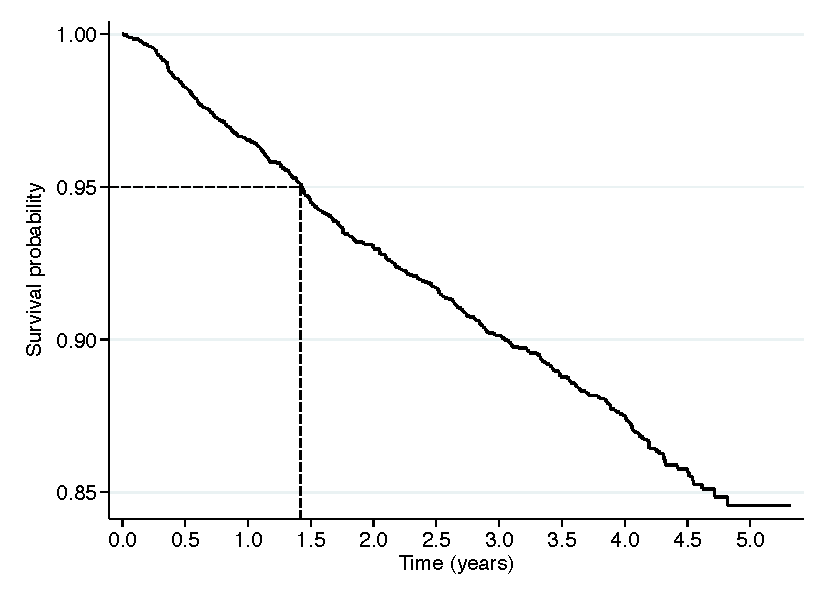
\includegraphics[width=.8\linewidth]{figures/kmpercentile.pdf}
\end{center}
\caption[Survival curve and 5th survival percentile]{Non-parametric survival curve estimate for all the women enrolled in the HERS trial (solid line) \citep{hulley_randomized_1998}. The dashed line illustrates the 5th survival percentile (around 1.4 years).}
\label{fig:kmpercentile}
\end{figure}

More formally, the $100p$-th survival percentile is defined as:
\begin{equation*}
Q_T(p) =  \inf \left\{ t: \Pr\left(T \le t\right) \ge p \right\}.
\end{equation*}
The function $Q_T(\cdot)$ is the quantile function, and is defined as that function such that $1-S\left(Q_T(p)\right) = F\left(Q_T(p)\right) = p$, where $F(\cdot)$ is the c.d.f. of $T$ introduced at the beginning of section \ref{section:basicstatconcepts}. Of note, not all the survival percentiles are always estimable. It is not possible for example to calculate the 25th survival percentile for the survival curves presented in figure \ref{fig:kmpercentile}. This is because at the end of the follow-up time, only around 15\% of the individuals  had experienced the event of interest (coronary heart disease). However, all the percentiles up to the 15th are estimable. For example, the 5th survival percentile obtained from the Kaplan-Meier estimate of the survival curve was around 1.4 years (dashed line).

One might want to estimate the $100p$-th survival percentile conditional on a given covariate vector $\mathbf{x}$. In this case, the definition of survival percentiles easily extends to:
\begin{equation*}
Q_{T}(p|\mathbf{x}) =  \inf \left\{ t: \Pr\left(T \le t|\mathbf{x}\right) \ge p \right\},
\end{equation*}
and comparisons between groups of individuals (for example, exposed and unexposed) in terms of time elapsed before a certain proportion of individuals has experienced the event can be made. For example, in figure \ref{fig:phnophsurvcurve}, the 5th survival percentile for those women in the active treatment arm (red dashed line) was around 1.3 years, whereas the same percentile was around 1.6 years for those women in the placebo arm (blue dashed line). As a result, the 5th PD between the placebo and treatment arm was 0.3 years. On the other hand, the 15th PD was practically equal to 0 years.

A statistical method that combines the flexibility of a modeling approach with the simplicity of focusing directly on survival percentiles is quantile regression for censored data. 

\subsubsection{Quantile regression for censored data}

The idea behind quantile regression for censored data is to link the conditional $100p$-th survival percentile $Q_{T_i}(p|\mathbf{x}_i)$ to the covariate vector $\mathbf{x}_i=\left(x_{i1},\ldots,x_{ik}\right)$ (generally including an intercept) though a linear, additive model. In particular:
\begin{equation}
Q_{T_i}(p|\mathbf{x}_i) = \mathbf{x}_i^\top\boldsymbol{\beta}(p) = \sum_{j=0}^k \beta_j(p)  x_{ij}.
\label{eq:quantilemod}
\end{equation}

Some considerations regarding this model are necessary. First, the notation $\boldsymbol{\beta}(p)$ underlines the important characteristic that the model coefficients are not constrained to be equal for different survival percentiles. Therefore, no assumptions similar to the proportionality of the hazards are made.

Second, the linear predictor $\mathbf{x}_i^\top\boldsymbol{\beta}(p)$ can include flexible transformations of continuous covariates (such as splines of fractional polynomials), product terms, and the like. This model is perfectly suited for the analysis of epidemiologic data, where it is important to be able to model continuous covariates and adjust for confounding. 

Third, by estimating multiple percentiles, one can thoroughly describe the distribution of $T$, conditionally on $\mathbf{x}$.

Fourth, the interpretation of the coefficients is particularly useful and straightforward, and it is strictly related to how one would interpret the coefficients of a classical linear regression. For example, just like in linear regression one would interpret a coefficient for a continuous variable $z$ as ``the change in the mean response variable for every 1-unit increase in $z$, adjusting for the other covariates in the model'', the interpretation of a similar coefficient from a quantile regression for survival data is ``the change in the $100p$-th survival percentile for every 1-unit increase in $z$, adjusting for the other covariates in the model''. The model coefficients are, in other words, PDs (and therefore absolute measures of association).\footnote{With the usual exception regarding the coefficient for the intercept, for the product terms, and for splines or other non-linear transformations of continuous variables.} 

Lastly, and most importantly, the model coefficients are now expressed in the metric of time, which means that they provide an intuitive measure of association between the covariates and the event of interest. This in contrast with the HRR, which is a dimensionless measure of association and possibly more difficult to interpret \citep{uno_moving_2014}.

Different methods have been proposed to deal with the model-based estimation of conditional percentiles when data is censored \citep{powell_censored_1986, portnoy_censored_2003, peng_survival_2008, wang_locally_2009, bottai_laplace_2010}. A description of the methods by Powell, Portnoy, and Peng and Huang can be found in \citet{koenker_censored_2008}. In this thesis and in \citetalias{bellavia_using_2015}, however, we will deal with the approach developed by \citet{bottai_laplace_2010} and known as `Laplace regression'.


\subsubsection{Laplace regression}

Re-introducing the notation used before, let $Y_i=\min(T_i,C_i)$ be the observed survival time measured on the $i$-th out of $n$ individuals. Moreover, let $d_i$ be indicator variable which takes value 1 if the survival time $Y_i$ is not censored and value 0 otherwise.

Assume that
\begin{equation}
T_i = \mathbf{x}_i^\top\boldsymbol{\beta}(p) + \epsilon_i,
\label{eq:laplacemodel}
\end{equation}
where $\mathbf{x}_i$ is the covariate vector, $\boldsymbol{\beta}(p)$ is the vector of unknown model coefficients, and $\epsilon_i$ are independently and identically distributed errors that follow a standard Laplace distribution, which is equivalent to an asymmetric Laplace (AL) distribution with location parameter 0 and scale parameter 1. For any given $p$, the $p$-th quantile of the conditional distribution of $T_i$ given $\mathbf{x}_i$ is $\mathbf{x}_i^\top\boldsymbol{\beta}(p)$ --- that is, $Q_{T_i}(p|\mathbf{x}_i) = \Pr(T_i \le \mathbf{x}_i^\top\boldsymbol{\beta}(p) | \mathbf{x}_i) = p$ \citep{bottai_laplace_2010}.

The AL distribution has a location parameter $\mu(p)$ and a scale parameter $\sigma(p)$. This notation underlines the fact that, in the specific situation presented in this thesis, $p$ is not a parameter to be estimated, rather it is treated as fixed. The AL distribution has the following p.d.f.:
\begin{equation}
f_{\textrm{AL}}\left(s\right) = \frac{p\left(1-p\right)}{\sigma(p)}\exp\left(-\frac{s-\mu(p)}{\sigma(p)}\left[p-I\left(s\le\mu(p)\right)\right] \right),
\label{eq:ald}
\end{equation}
where $\sigma(p)>0$, $-\infty < \mu(p) < +\infty$, and $I(\cdot)$ is the indicator function \citep{yu_threeparameter_2005}.

Therefore, since the asymmetric Laplace in (\ref{eq:ald}) is a location-scale family of densities, $T_i$ follows an AL distribution with p.d.f conditional to $\mathbf{x}_i$ equal to:
\begin{equation}
f_{\textrm{AL}}\left(t_i|\mathbf{x}_i\right) = \frac{p\left(1-p\right)}{\sigma(p)}\exp\left(-\frac{t_i-\mathbf{x}_i^\top\boldsymbol{\beta}(p)}{\sigma(p)}\left[p-I\left(t_i\le\mathbf{x}_i^\top\boldsymbol{\beta}(p)\right)\right] \right),
\label{eq:pdf}
\end{equation}
and c.d.f.
\begin{align}
\begin{split}
F_{\textrm{AL}}\left(t_i|\mathbf{x}_i\right) = &\exp\left(-\frac{t_i-\mathbf{x}_i^\top\boldsymbol{\beta}(p)}{\sigma(p)}\left[p-I\left(t_i\le\mathbf{x}_i^\top\boldsymbol{\beta}(p)\right) \right] \right) \left[p-I\left(t_i>\mathbf{x}_i^\top\boldsymbol{\beta}(p)\right)\right]  \label{eq:cdf} \\  
&+ I\left(t_i>\mathbf{x}_i^\top\boldsymbol{\beta}(p)\right)
\end{split}
\end{align}
as derived by \citet{bottai_laplace_2010}. The subscript AL in $f_{\textrm{AL}}(\cdot)$ and $F_{\textrm{AL}}(\cdot)$ is used to distinguish these functions from the p.d.f. and c.d.f. of $T$, respectively.  Heteroskedasticity of the error term can be accommodated by allowing the scale parameter $\sigma(p)$ to depend on a vector of covariates.

The contribution to the likelihood function $L$ of an uncensored observation ($d_i=1$) is given by the p.d.f. in (\ref{eq:pdf}) evaluated at the observed survival time $y_i$ --- that is $L_i=f_{\textrm{AL}}(y_i)$. On the other hand --- under the assumption of non-informative censoring conditionally on $\mathbf{x}_i$ --- a censored observation ($d_i=0)$  carries only the information that his/her event time $t_i$ is larger than $y_i$. The contribution to the likelihood function is therefore $L_i=1-F_{\textrm{AL}}(y_i)$. Consequently, the likelihood function is proportional to:\footnote{Note that this way of constructing the likelihood function also applies to parametric PH models under conditional independent right-censoring. See for example \citet[chapter~5]{lawless_statistical_2003} or \citet[chapter~3]{kalbfleisch_statistical_2002}.}
\begin{equation*}
L(\boldsymbol{\beta}(p), \sigma(p);y_i, \mathbf{x}_i, d_i)= \prod_{i=1}^n f_{\textrm{AL}}(y_i|\mathbf{x}_i)^{d_i} \left(1-F_{\textrm{AL}}(y_i|\mathbf{x}_i)\right)^{(1-d_i)}.
\end{equation*}

The log-likelihood function is obtained as usual by taking the logarithm of the likelihood:
\begin{equation}
l(\boldsymbol{\beta}(p), \sigma(p);y_i, \mathbf{x}_i, d_i)= \sum_{i=1}^n \left[ d_i \log f_{\textrm{AL}}(y_i|\mathbf{x}_i) + \left(1-d_i\right) \log \left(1-F_{\textrm{AL}}(y_i|\mathbf{x}_i)\right) \right].
\label{eq:logliklap}
\end{equation}

Lastly, by substituting equations (\ref{eq:pdf}) and (\ref{eq:cdf}) in (\ref{eq:logliklap}), and after some algebraic manipulations, the log-likelihood function becomes:
\begin{align}
\begin{split}
l(\boldsymbol{\beta}(p), \sigma(p)&;y_i, \mathbf{x}_i, d_i)= d_i \left[ -\frac{y_i-\mathbf{x}_i^\top\boldsymbol{\beta}(p)}{\sigma(p)} \left(p-I\left(y_i\le\mathbf{x}_i^\top\boldsymbol{\beta}(p)\right) \right) + \log\frac{p\left(1-p\right)}{\sigma(p)} \right] \\ 
&+\left(1-d_i\right) I\left(y_i\le\mathbf{x}_i^\top\boldsymbol{\beta}(p)\right) \log\left[1 - p \exp\left( (1-p)  \frac{y_i-\mathbf{x}_i^\top\boldsymbol{\beta}(p)}{\sigma(p)} \right) \right] \\ 
&+ \left(1-d_i\right) \left(1-I\left(y_i\le\mathbf{x}_i^\top\boldsymbol{\beta}(p)\right)\right) \left[ \log \left(1-p\right) - p \frac{y_i-\mathbf{x}_i^\top\boldsymbol{\beta}(p)}{\sigma(p)} \right].
\label{eq:logliklapexpanded}
\end{split}
\end{align}

The maximum likelihood (ML) estimators for the model parameters $\hat{\boldsymbol{\beta}}(p)$ and $\hat{\sigma}(p)$ are defined as the maximizers of the log-likelihood (\ref{eq:logliklapexpanded}), which can be directly maximized using, for example, the gradient search algorithm recently proposed by \citet*{bottai_gradient_2015}. %This algorithm showed remarkable computational speed both in a simulation study and in real-data applications. This maximization algorithm overcomes the limitations of the Nelder-Mead algorithm used in the original paper on Laplace regression \citep[see also][]{bottai_authors_2011}.
Inference on the parameters can be obtained through bootstrapping, as initially proposed in \citet{bottai_laplace_2010}, or following standard asymptotic theory, as shown in  \citet{bottai_command_2013}.

Note that when censoring occurs with zero probability before the survival percentile being estimated, Laplace regression reduces to traditional quantile regression \citep{bottai_laplace_2010}.

Thanks also to the development of a user-friendly command to estimate Laplace regression with Stata \citep{bottai_command_2013}, quantile regression for censored data has been repeatedly employed in the recent years to analyze survival data in epidemiology \citep[see, for example,][]{rizzuto_lifestyle_2012, bellavia_sleep_2014, rahman_relationship_2014}. %For example, quantile regression was employed to evaluate the association between physical activity and the 8th percentile of heart failure--free survival time \citep{rahman_relationship_2014}, or between the 15th percentile of time-to-death and physical activity by categories of sleep duration \citep{bellavia_sleep_2014}. 
Moreover, quantile regression for censored data has been proposed as a tool to evaluate additive interaction in survival analysis \citep{bellavia_evaluating_2016}, and to estimate conditional and marginal survival curves \citep{bellavia_adjusted_2015}. 

Lastly, we recently proposed to use quantile regression for censored data --- and in particular Laplace regression --- as a flexible and intuitive approach to estimate survival percentiles of age at the event (for example, age at prostate cancer death). This extends the use of this statistical tool, especially in epidemiologic research. In fact, investigators are often more interested in describing the distribution of age at the event for a group of individuals rather than the distribution of time elapsed between some arbitrary baseline event (for example, filling in a questionnaire) and the occurrence of a disease \citepalias{bellavia_using_2015}. 


\subsection{Risk and rate advancement periods}

One of the most interesting features of quantile regression is probably that the exposure-outcome association is expressed in the metric of time as PDs. %, which makes PDs very appealing in communicating study results. 
Other methods have been proposed in the literature to express the impact of an exposure  on the time of disease onset, such as risk and rate advancement periods (RAP) or `expected years of (disease-free) life lost'.

RAP, in particular, was introduced by \citet*{brenner_risk_1993} to measure the age difference at which exposed subjects reach the same rate/risk as unexposed subjects, assuming a monotonic increase in event rate/risk over age, independence of the outcome of interest from competing risks, and conditional on disease-free survival to some baseline age. In this section we will refer to the rate advancement period only.\footnote{To be consistent with the previous sections, the notation used in this thesis is slightly different from that used in \citetalias{discacciati_interpretation_2015}.} The risk advancement period is defined in a similar fashion and is presented in \citetalias{discacciati_interpretation_2015}.

This measure has been recently given special attention by the CHANCES consortium,\footnote{\href{http://www.chancesfp7.eu}{\texttt{http://www.chancesfp7.eu}}} which is an international pooling project of primary data from cohort studies [including the Cohort of Swedish Men (COSM), see section~\ref{section:cosm}] \citep{boffetta_consortium_2014}.  The quantification of RAP to assess the impact of health-related characteristics on chronic diseases (including cancer) and overall mortality is the principal research aim of published papers \citep{mons_impact_2015, muezzinler_smoking_2015} and research proposals \citetext{Orsini, personal communication}.

\subsubsection{Definition}

Suppose one wants to assess in a cohort study the association between an exposure $e$ and the rate $R$ of a binary event of interest $d$. Let $h(a,e,\mathbf{c})$ be the hazard of the outcome $d$ at baseline age $a$ among those at exposure level $e$ with a fixed covariate vector $\mathbf{c}=(c_1, \ldots, c_k)$. Suppose also that one is interested in two fixed exposure levels in particular, say $e_0$ and $e_1$. For any given baseline age $a_1$, the idea behind the RAP is to seek the earliest age $a_0$ such that:
\begin{equation}
h(a_0, e_0, \mathbf{c}) = h(a_1, e_1, \mathbf{c}).
\label{eq:definitionrap}
\end{equation}

If an $a_0$ satisfying the preceding equation exists, one can define the difference in baseline ages $a_0-a_1$ as the RAP among $e_1$-exposed as compared with $e_0$-exposed, starting from the baseline age $a_1$. The existence of a unique value $a_0$ (and therefore the uniqueness of RAP) is guaranteed by the assumption that the hazard function of $d$ increases monotonically with age, given $e$ and $\mathbf{c}$.

For example, if RAP is equal to 20 years starting from a baseline age of 40 years, then $e_1$-exposed individuals that were 40 years of age at baseline experienced the same rate of the disease than $e_0$-exposed subjects who were 60 years of age at baseline.

\subsubsection{The form of risk and rate advancement periods under PH models}

RAP can be estimated parametrically directly from PH models. In fact, by taking the logarithm of both sides of equation \ref{eq:phmodels}, one obtains:
\begin{equation}
\log\left[h(t|\mathbf{x})\right] = \log \left[ h_0(t) \right] +\mathbf{x}^\top\boldsymbol{\beta} = \log \left[ h_0(t) \right] + \beta_1 e + \beta_2 g(a) + \sum_{i=1}^k \beta_{i+2}c_i,
\label{eq:parametricrap}
\end{equation}
where $g(\cdot)$ is a smooth, monotonically increasing function of baseline age. The usual default transform of age is the identity function $g(a) = a$.

Under the assumptions previously introduced, a group of $e_1$-exposed individuals who have a certain rate at baseline age $a_1$ would be expected to have reached the same rate at age $a_0$, had they been $e_0$-exposed, given that all the other covariates $\mathbf{c}$ are kept constant. Therefore, according to (\ref{eq:parametricrap}),
\begin{align}
\begin{split}
\log \left[ h_0(t) \right] + \beta_1 e_1 + \beta_2 g(a_1) + \sum_{i=1}^k \beta_{i+2}c_i &= \log \left[ h_0(t) \right] + \beta_1 e_0 + \beta_2 g(a_0) + \sum_{i=1}^k \beta_{i+2}c_i \\
\beta_1 e_1 + \beta_2 g(a_1) &=  \beta_1 e_0 + \beta_2 g(a_0). \label{eq:rapsimplified}
\end{split}
\end{align}

Thus, if $e_1-e_0=1$, $\beta_2 \neq 0$, and $g(\cdot)$ is the identity function,
\begin{equation}
\mathrm{RAP} = a_0 - a_1 = \frac{\beta_1}{\beta_2},
\label{eq:para_rap}
\end{equation}
which is the RAP for a 1-unit increase in $e$, expressed in the time scale of $a$ (for example years, if baseline age is expressed in years).

Note that if $g(\cdot)$ is not the identity function, RAP is no longer constant over baseline age and it will depend on $a_1$. For example, if $g(a) = \log(a)$, RAP becomes
\begin{equation}
\mathrm{RAP}(a_1) = a_0 - a_1 = \left[ \exp \left( \frac{\beta_1}{\beta_2} \right) - 1 \right] a_1.
\label{eq:para_log_rap}
\end{equation}

Unfortunately, this measure has been misinterpreted in  studies, commentaries, and editorials published in major epidemiologic and medical journals. Moreover, important aspects regarding RAP estimation have often been overlooked. These aspects are covered in detail in \citetalias{discacciati_interpretation_2015}.


